% !TEX encoding = UTF-8 Unicode
\RequirePackage{fix-cm}
\documentclass[a4paper,10pt,UTF8]{paper}
%\documentclass[a4paper,10pt,UTF8]{ctexart}

\usepackage[english]{babel}
\usepackage{fancyhdr,array,lastpage,amsmath,mathtools,enumitem,graphicx,multirow,tocbibind,longtable,makecell,varwidth,titlesec,bm,booktabs,comment,minted, tabularx}
\usepackage{enumitem}
\usepackage{hyperref}
\hypersetup{hidelinks}


\usepackage[left=2.54cm,right=2.54cm,top=2.54cm,bottom=2.54cm]{geometry}
\usepackage[font=footnotesize,labelfont=bf]{caption}
\usepackage{tikz,flowchart}
\usepackage{ctex}
\usepackage{xeCJK}%中文字体
\usetikzlibrary{shapes,shapes.geometric,arrows,matrix,calc}
\usetikzlibrary{circuits.logic}

% \usetikzlibrary{circuits.logic.custom}
\usetikzlibrary{circuits.logic.IEC}
\usetikzlibrary{shadows}
\usepackage{listings}
\usepackage[Q=yes]{examplep}
\usepackage{fancyhdr}
\usepackage{alphalph}
\usepackage{indentfirst}

% \setCJKsansfont{黑体}
\setmainfont{PingFang SC}
\setCJKmainfont{PingFang SC}
\setCJKsansfont{PingFang SC}

\usepackage[left=2.54cm,right=2.54cm,top=2.54cm,bottom=2.54cm]{geometry}
\usepackage[font=footnotesize,labelfont=bf]{caption}
\usepackage{tikz,flowchart}
\usepackage{ctex}
\usetikzlibrary{shapes,shapes.geometric,arrows,matrix,calc}
\usetikzlibrary{circuits.logic}
% \usetikzlibrary{circuits.logic.custom}
\usetikzlibrary{circuits.logic.IEC}
\usetikzlibrary{shadows}
\usepackage{listings}
\usepackage[Q=yes]{examplep}
\usepackage{fancyhdr}
\usepackage{alphalph}
\usepackage{indentfirst}

\newenvironment{sol}
  {\par\vspace{2mm}\noindent{\bf Solution}. }

\lstset{escapeinside=``, breaklines=true, frame=none, extendedchars=false, basicstyle=\ttfamily, showstringspaces=false}


\setlength{\parindent}{2em}
\setlength{\parskip}{1.5ex plus 0.5ex minus 0.2ex}
\linespread{1.1}

\bibliographystyle{plain}

\numberwithin{equation}{section}
\numberwithin{figure}{section}

\usepackage{karnaugh}
\usepackage{circuitikz}


\setcounter{secnumdepth}{3}
\setcounter{tocdepth}{3}

\title{华东师范大学计算机科学技术系上机实验报告}

\begin{document}
\pagestyle{fancy}
\chead{\small\color{gray}华东师范大学计算机科学技术系上机实验报告}
\lhead{}
\rhead{}
\makeatletter
\def\headrule{{\if@fancyplain\let\headrulewidth\plainheadrulewidth\fi%
	\color{gray}\hrule\@height 0.2pt\@width\headwidth}
	\vspace{6mm}}
\makeatother

\newcommand{\HRule}{\rule{\linewidth}{1mm}}
\newcommand{\dai}{\textbf{Dais-CMX16$^+$}}

{\center {\huge \bfseries \LARGE{华东师范大学计算机科学技术系上机实验报告}} \\ [0.8cm]
	
	\small{
		\begin{minipage}[t]{.32\linewidth}
			\textbf{课程名称:}计算机组成与结构实践\\
			\textbf{指导教师:}金健\\
			\textbf{上机实践名称:} 中断控制实验\\
			\textbf{实践编号:}实验 6
		\end{minipage}
		\begin{minipage}[t]{.32\linewidth}
			\textbf{年级:}17 级\\
			\textbf{姓名:}朱桐\\
			\textbf{学号:}10175102111\\
			\textbf{组号:}A
		\end{minipage} 
		\begin{minipage}[t]{.32\linewidth}
			\textbf{上机实践成绩:} \\
			\textbf{创新实践成绩:} \\
			\textbf{上机实践日期:}2019/09/20\\
			\textbf{上机实践时间:}2 学时\\
		\end{minipage}
	}
	\HRule \\[0.5cm]
}
\section{实验目的}

\begin{enumerate}
	\item 掌握中断的控制方法。
\end{enumerate}

\section{实验设备}

\dai

\section{实验内容}

分别开关 IEQ,IAQ,INQ


\section{实验原理}

下图 \ref{fig:1} 分别表示:一般指令,和支持中断的指令

\begin{figure}[h]
	\centering
	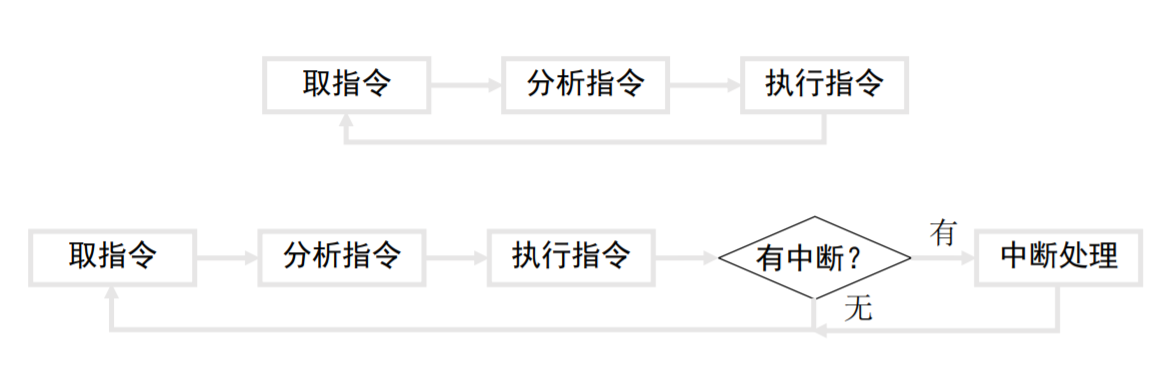
\includegraphics[width=0.9\textwidth]{1.PNG}
	\caption{中断发生}
	\label{fig:1}
\end{figure}
本质区别:
\begin{enumerate}
	\item 支持中断的系统,机器指令对应的微程序执行完,要判断是否有中断(INQ=0)
	\item 中断请求标志INQ低电平有效,0表示有中断请求
\end{enumerate}

所谓中断就是指处理机暂时终止执行现行程序而转去处理更加紧迫的事件服务程序,待处理
机完毕后再自动返回执行原来的程序过程。
按图 2-4-12 所示,本系统提供了一个单级中断硬件机制,由中断请求源 INT、中断允许标
志 IEQ 和中断响应标志 IAQ 组成。
微程序控制器每执行一条机器指令之后,先查询中断允许标志 IEQ,如果 IEQ 为 0,则继续
执行下一条机器指令,若检测到 IEQ 为 1,则强制转入微程序控制器的 0003h 号单元执行中断响
应微服务。期间程序首先置位中断响应标志 IAQ,其次执行当前 PC 的进栈操作,然后按照机器
程序的要求随机定义中断向量,把中断服务程序入口地址装入程序计数器 PC 中,转入中断服务
子程序的执行。
遇 RET 指令,执行中断服务返回微操作,清除中断服务响应标志 IAQ,把栈顶所指单元的
内容装入程序计数器 PC 中,恢复执行被中断的机器程序。

\subsection{控制电路}

如图 \ref{fig:2} 为控制电路

\begin{figure}[h]
	\centering
	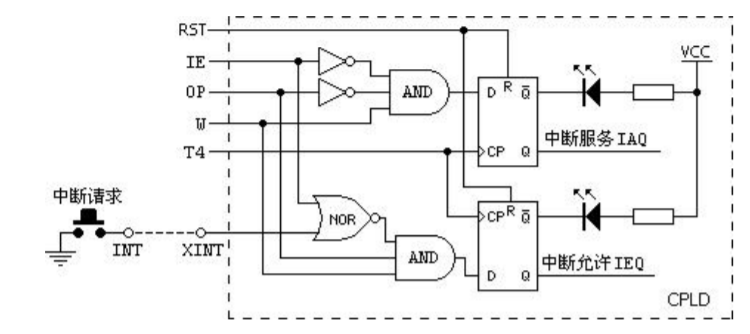
\includegraphics[width=0.9\textwidth]{2.PNG}
	\caption{中断控制电路}
	\label{fig:2}
\end{figure}

\subsection{控制格式}

\subsubsection{终端控制请求IEQ}

\begin{center}
	\begin{tabular}{|c|c|c|c|c|c|c|}
		\hline
		K7 & K6 & K3 & 按钮 & 节拍     & 功能              & 说明             \\ \hline
		OP & W  & Ie & INT    & T4         &                     &                    \\ \hline
		0  & 0  & 1  & 0      & $\uparrow$ & 1 $\rightarrow$ IEQ & 锁存中断请求 \\ \hline
		0  & 1  & 1  & X      & $\uparrow$ & 0 $\rightarrow$ IEQ & 清除中断请求 \\ \hline
		  
	\end{tabular}
\end{center}

说明:上表中的中断请求 INT 由【中断】按钮模拟产生,T4 节拍在手动状态由【单拍】按
钮模拟产生。

\subsubsection{中断响应控制}

\begin{center}
	\begin{tabular}{|c|c|c|c|c|c|c|}
		\hline
		K7 & K6 & K3 & 按钮 & 节拍     & 功能              & 说明       \\ \hline
		OP & W  & Ie & INT    & T4         &                     &              \\ \hline
		1  & 0  & 1  & 0      & $\uparrow$ & 1 $\rightarrow$ IAQ & 中断响应 \\ \hline
		1  & 1  & 1  & 0      & $\uparrow$ & 0 $\rightarrow$ IAQ & 中断推出 \\ \hline
	\end{tabular}  
\end{center}

\section{实验步骤}

本次实验相对简单,按照步骤操作即可

\section{调试过程、结果与分析}

\begin{figure}[h]
	\centering
	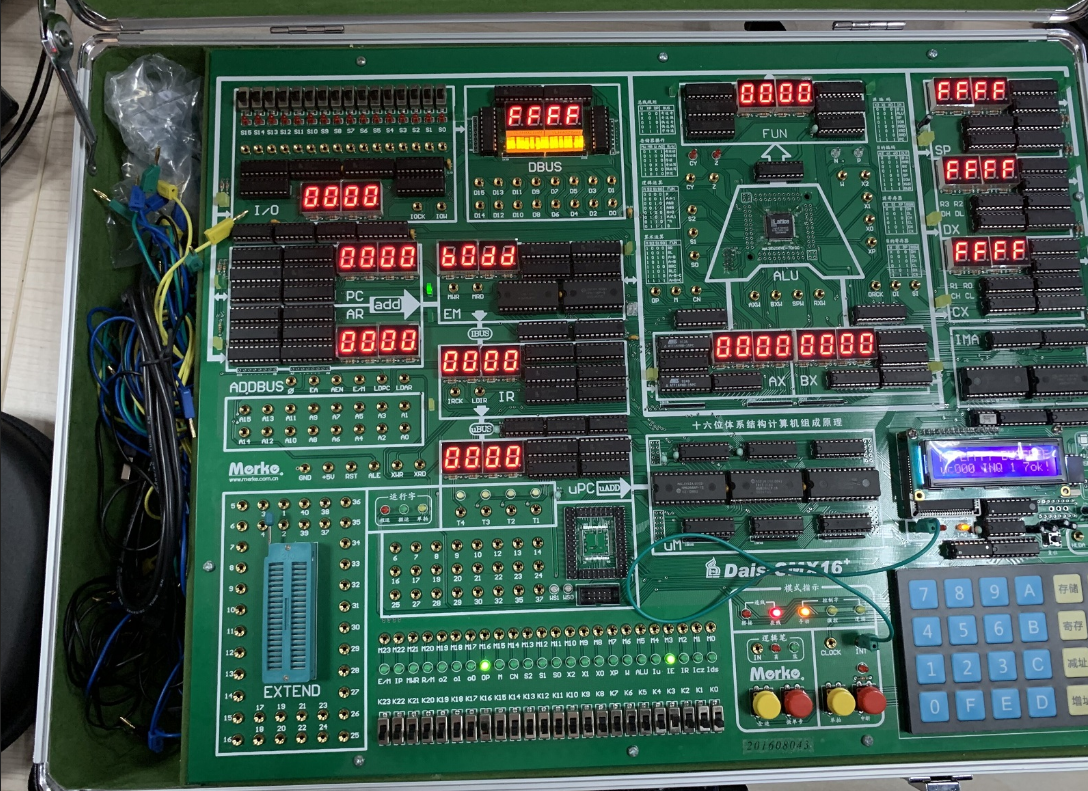
\includegraphics[width=0.7\textwidth]{3.png}
	\caption{实验结果}
\end{figure}

\begin{figure}[h]
	\centering
	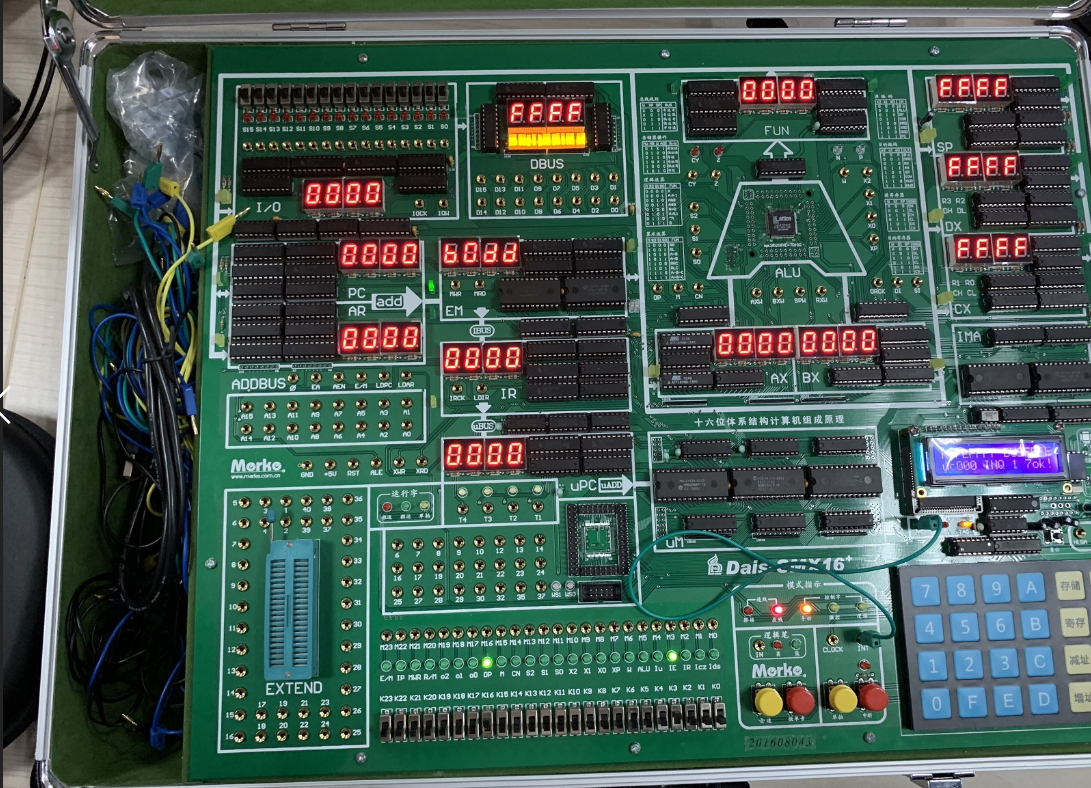
\includegraphics[width=0.7\textwidth]{4.png}
	\caption{实验结果}
\end{figure}


\section{总结}

本次实验比较简单,没有碰到什么问题

\section{附件}

\end{document}
